\documentclass{article}
\usepackage[margin=7.5mm,paperwidth=10.5cm,paperheight=21.0cm]{geometry}
\usepackage[T1]{fontenc}
\usepackage[utf8]{inputenc}
\usepackage{graphicx}
\usepackage{xcolor}
\usepackage{listings}
\usepackage{multicol}
\usepackage{pgfornament}
\usepackage{ebgaramond}
\usepackage{pgfpages}
\usepackage{tikz}
\usepackage{tikzpagenodes}
\usepackage[a4,cam,cross]{crop}
\pgfpagesdeclarelayout{christmas}{
    \edef\pgfpageoptionheight{\the\paperheight}
    \edef\pgfpageoptionwidth{\the\paperwidth}
    \edef\pgfpageoptionborder{0pt}
}{  \pgfpagesphysicalpageoptions{
        logical pages=2,
        physical height=29.7cm,
        physical width=21.0cm
    }\pgfpageslogicalpageoptions{2}{
        border shrink=\pgfpageoptionborder,
        resized width=10.5cm, resized height=21.0cm,
        center=\pgfpoint{.25\pgfphysicalwidth}{.5\pgfphysicalheight}
    }\pgfpageslogicalpageoptions{1}{
        border shrink=\pgfpageoptionborder,
        resized width=10.5cm, resized height=21.0cm,
        center=\pgfpoint{.75\pgfphysicalwidth}{.5\pgfphysicalheight}
    }
}\pgfpagesuselayout{christmas}
\pagenumbering{gobble}
\definecolor{christmas}{HTML}{b12424}
\renewcommand{\c}[1]{{\color{christmas}#1}}
\lstset{
    language=TeX,
    morekeywords={begin,renewcommand,usepackage},
    basicstyle=\tiny\ttfamily,
    keywordstyle=\color{christmas},
    commentstyle=\color{darkgray}
}

% Source code also found on: https://github.com/Kamik423/christmas-card-2019
\begin{document}
\begin{tikzpicture}[remember picture, overlay]
    \node[anchor=north west] at (current page text area.north west) {%
        \pgfornament[width=1.5cm]{63}};
    \node[anchor=north east] at (current page text area.north east) {%
        \pgfornament[width=1.5cm, symmetry=v]{63}};
    \node[anchor=south west] at (current page text area.south west) {%
        \pgfornament[width=1.5cm,symmetry=h]{63}};
    \node[anchor=south east] at (current page text area.south east) {%
        \pgfornament[width=1.5cm,symmetry=c]{63}};
\end{tikzpicture}
\centering
% You are being loved <3
\vfill
{\Huge \c{F}rohe \c{W}eihnachten\\[5mm]}
{\Huge\c{\&}}\\[5mm]
{\Large einen guten \c{R}utsch ins neue \c{J}ahr}\\[5mm]
{\Large wünscht euch \c{H}ans.}\\

\vfill
\hspace{1cm}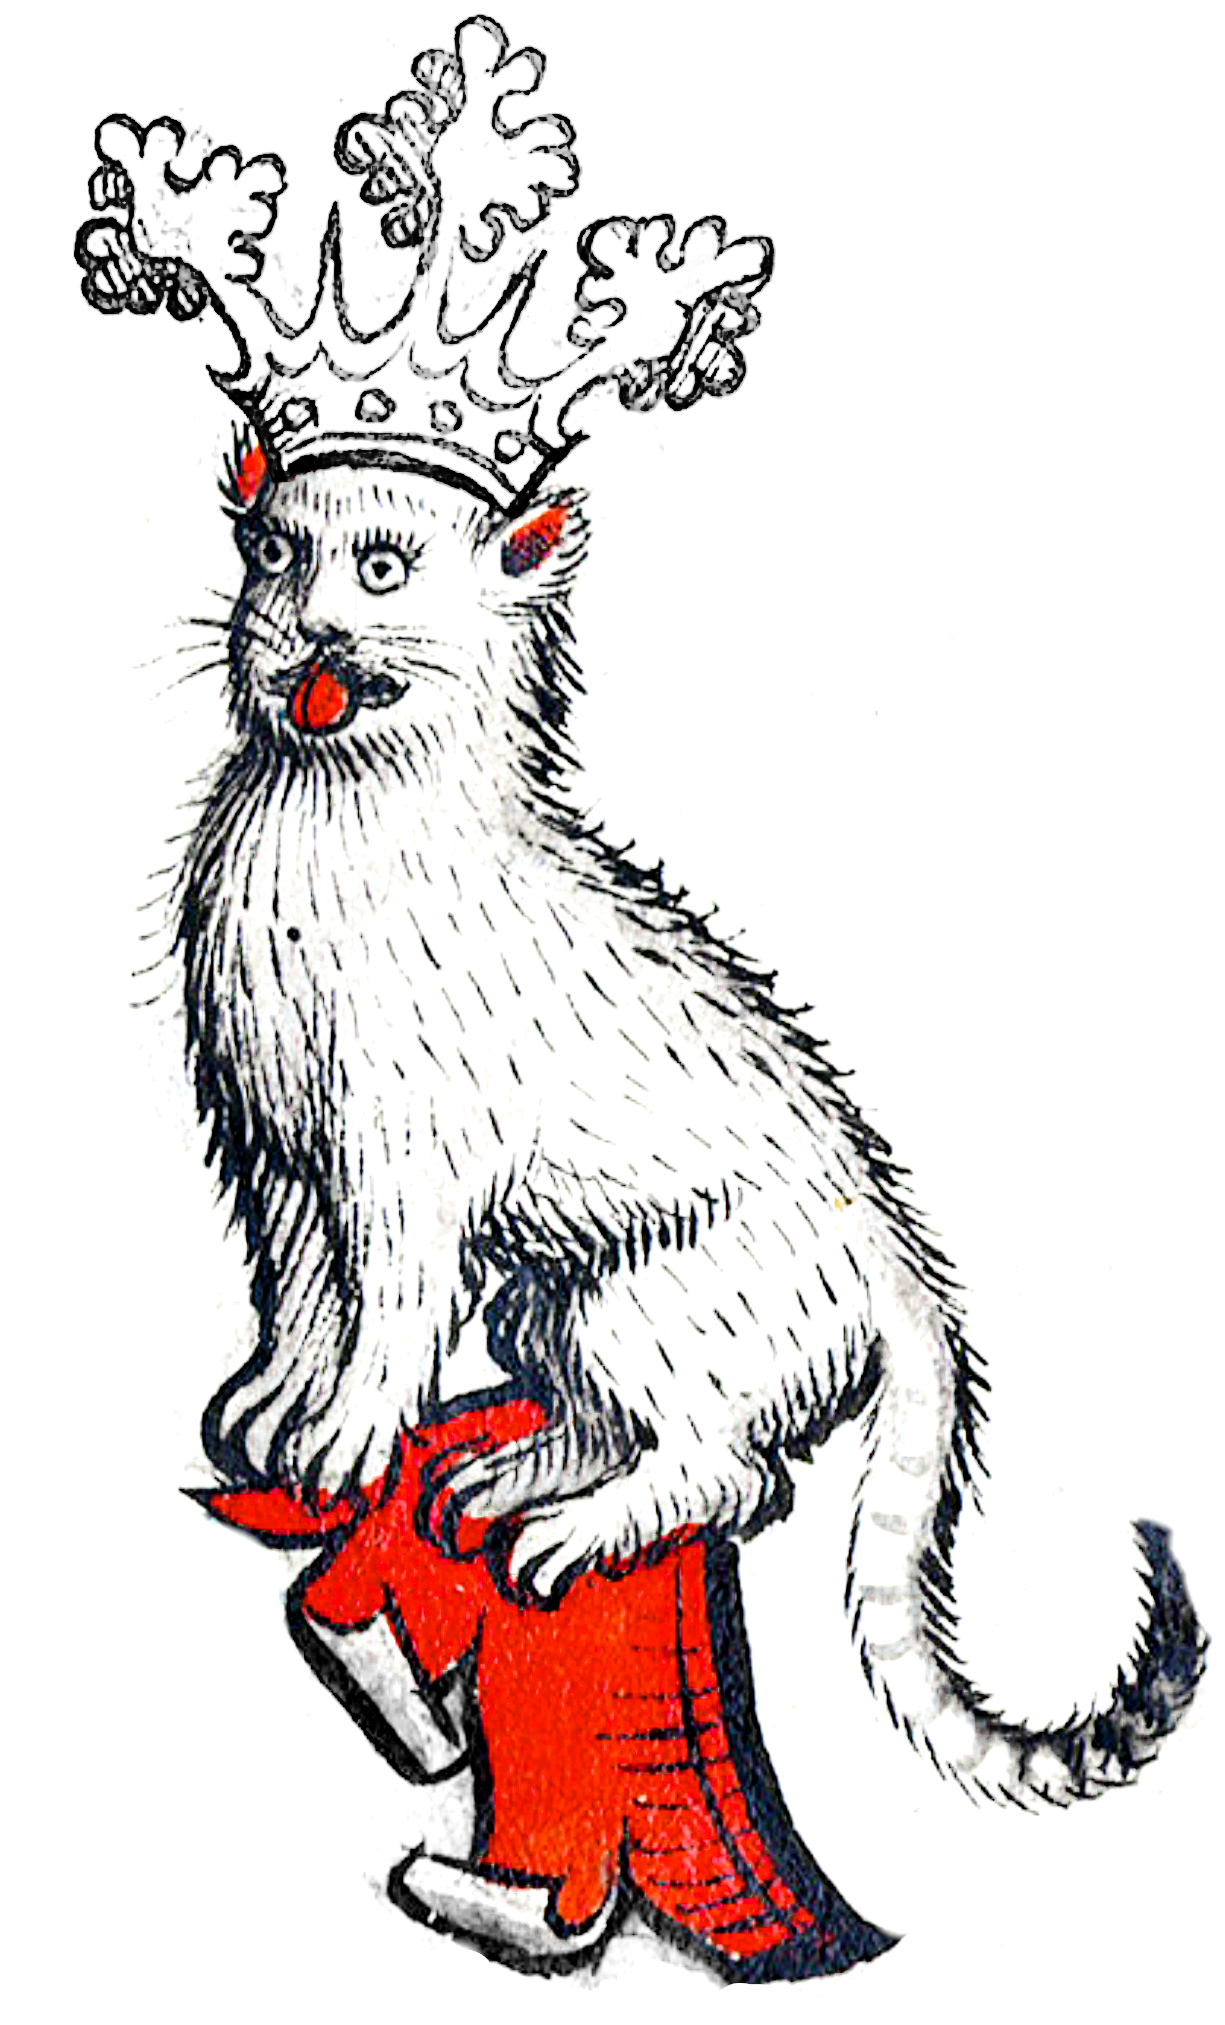
\includegraphics[width=6cm]{cat.png}
% Cat sourced from:
% https://www.reddit.com/r/MedievalCats/comments/e713ht/king_derpy/
% Edited version on:
% https://github.com/Kamik423/christmas-card-2019

\vfill
\begin{minipage}[c]{.8\textwidth}
    \centering
    \large
    \c{``}Give a man a fire and he's warm for a day, but set fire to him
    and he's warm for the rest of his life.\c{''}\\[5mm]
    \c{--}Sir Terry Pratchett
\end{minipage}

\vfill
\newpage %%%%%%%%%%%%%%%%%%%%%%%%%%%%%%%%%%%%%%%%%%%%%
\lstinputlisting{christmas-card-2019.tex}
\vfill Typeset by Hans in EBGaramond in \LaTeX.
\end{document}